\documentclass{standalone}\usepackage[utf8]{inputenc}\usepackage{tikz,fontenc,graphicx}\usepackage[pdftex]{hyperref}\hypersetup{pdfborder={0 0 0},breaklinks=true}\begin{document} \left( 
\{ p , p_{2} \},  \begin{array}{l} \scalebox{0.4}{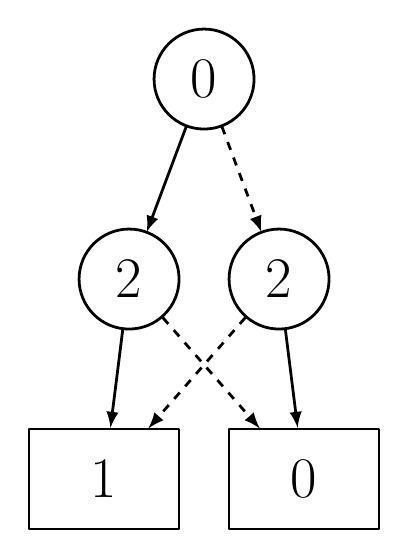
\begin{tikzpicture}[>=latex,line join=bevel,]
  \pgfsetlinewidth{1bp}
\huge%
\begin{scope}
  \pgfsetstrokecolor{black}
  \definecolor{strokecol}{rgb}{1.0,1.0,1.0};
  \pgfsetstrokecolor{strokecol}
  \definecolor{fillcol}{rgb}{1.0,1.0,1.0};
  \pgfsetfillcolor{fillcol}
  \filldraw (0.0bp,0.0bp) -- (0.0bp,180.0bp) -- (126.0bp,180.0bp) -- (126.0bp,0.0bp) -- cycle;
\end{scope}
\begin{scope}
  \pgfsetstrokecolor{black}
  \definecolor{strokecol}{rgb}{1.0,1.0,1.0};
  \pgfsetstrokecolor{strokecol}
  \definecolor{fillcol}{rgb}{1.0,1.0,1.0};
  \pgfsetfillcolor{fillcol}
  \filldraw (0.0bp,0.0bp) -- (0.0bp,180.0bp) -- (126.0bp,180.0bp) -- (126.0bp,0.0bp) -- cycle;
\end{scope}
  \pgfsetcolor{black}
  % Edge: n0 -> n1
  \draw [->] (56.601bp,144.94bp) .. controls (53.407bp,136.42bp) and (49.471bp,125.92bp)  .. (42.353bp,106.94bp);
  % Edge: n0 -> n2
  \draw [->,dashed] (69.399bp,144.94bp) .. controls (72.593bp,136.42bp) and (76.529bp,125.92bp)  .. (83.647bp,106.94bp);
  % Edge: n1 -> Top
  \draw [->] (33.729bp,71.831bp) .. controls (32.766bp,64.131bp) and (31.622bp,54.974bp)  .. (29.302bp,36.413bp);
  % Edge: n1 -> Bot
  \draw [->,dashed] (48.147bp,76.118bp) .. controls (56.146bp,66.976bp) and (66.863bp,54.728bp)  .. (83.072bp,36.204bp);
  % Edge: n2 -> Top
  \draw [->,dashed] (77.853bp,76.118bp) .. controls (69.854bp,66.976bp) and (59.137bp,54.728bp)  .. (42.928bp,36.204bp);
  % Edge: n2 -> Bot
  \draw [->] (92.271bp,71.831bp) .. controls (93.234bp,64.131bp) and (94.378bp,54.974bp)  .. (96.698bp,36.413bp);
  % Node: n0
\begin{scope}
  \definecolor{strokecol}{rgb}{0.0,0.0,0.0};
  \pgfsetstrokecolor{strokecol}
  \draw (63.0bp,162.0bp) ellipse (18.0bp and 18.0bp);
  \draw (63.0bp,162.0bp) node {0};
\end{scope}
  % Node: n1
\begin{scope}
  \definecolor{strokecol}{rgb}{0.0,0.0,0.0};
  \pgfsetstrokecolor{strokecol}
  \draw (36.0bp,90.0bp) ellipse (18.0bp and 18.0bp);
  \draw (36.0bp,90.0bp) node {2};
\end{scope}
  % Node: n2
\begin{scope}
  \definecolor{strokecol}{rgb}{0.0,0.0,0.0};
  \pgfsetstrokecolor{strokecol}
  \draw (90.0bp,90.0bp) ellipse (18.0bp and 18.0bp);
  \draw (90.0bp,90.0bp) node {2};
\end{scope}
  % Node: Top
\begin{scope}
  \definecolor{strokecol}{rgb}{0.0,0.0,0.0};
  \pgfsetstrokecolor{strokecol}
  \draw (54.0bp,36.0bp) -- (0.0bp,36.0bp) -- (0.0bp,0.0bp) -- (54.0bp,0.0bp) -- cycle;
  \draw (27.0bp,18.0bp) node {1};
\end{scope}
  % Node: Bot
\begin{scope}
  \definecolor{strokecol}{rgb}{0.0,0.0,0.0};
  \pgfsetstrokecolor{strokecol}
  \draw (126.0bp,36.0bp) -- (72.0bp,36.0bp) -- (72.0bp,0.0bp) -- (126.0bp,0.0bp) -- cycle;
  \draw (99.0bp,18.0bp) node {0};
\end{scope}
%
\end{tikzpicture}} \end{array}
 , \begin{array}{l}
 \varnothing  \\
 \{ p_{2} \}\end{array}
 \right) , \{ p , p_{2} \}\end{document}